% N-integrals by R^n - \underset{R^n}{ \int \cdots \int}


\begin{center}
	\Huge \textbf{Собственно, матстат...}
\end{center}
\section{Функції від випадкових величин (векторів)}
Для дискретної випадкової величини $\xi$: $\eta = \phi (\xi) \Rightarrow \eta$ - ДВВ. \\
Припустимо, що $\varphi$ - неперервно диференційована. $\xi$ - асолютно неперервна зі щільністю $f_{\xi}(x)$. Розглядаємо $ \eta = \varphi(\xi) $:

\begin{boxteo}
    Нехай $\varphi$ - взаємно-однозначна (бієкція на області значень), та її обернена $\psi$ є неперервно диференційована. (Дифеоморфізм). Тоді:
    $$
    f_{\eta} (y) = \begin{cases}
    \left| \psi '(y) \right| \cdot  f_{\xi }(\psi (y)), & y \in E_{\varphi}\\
        0 & y \notin E_{\varphi}
    \end{cases} = f_{\xi} (\psi (y)) \cdot \left| \psi'(y) \right| \cdot \mathbb{I}_{E_{\varphi}}(y)
    $$
\end{boxteo}

\begin{proof}
Розглядаемо множину B.
$$  \int\limits_{B }^{ }{ f_{\eta} (y)dy} = \mathbb{P} \left\lbrace \eta \in B \right\rbrace =
\mathbb{P} \left\lbrace \varphi(\xi) \in B \right\rbrace = \mathbb{P} \left\lbrace \xi \in \phi^{-1} (B) \right\rbrace =  \int\limits_{\phi^{-1} (B)}^{}{f_{\xi}(x)dx} =
$$

$$
= \left| \begin{gathered}
  \varphi(x) = y \\
  x = \psi(y) \\
  J = \psi'(y) = J_{\psi}
\end{gathered} \right|  =  \int\limits_{B \cap E_{\varphi}}^{ }{ f_{\xi} (\psi (y)) \cdot \left| J_{\psi} (y)  \right| dy} =  \int\limits_{B}^{ }{f_{\xi} (\psi (y)) \cdot \left| \psi'(y) \right| \cdot \mathbb{I}_{E_{\varphi}}(y)dy}
$$
\end{proof}
\begin{boxteo}
Нехай $\phi$ не є ін'єкцією, але ''розпадається'' на декілька таких.
$$
\begin{gathered}
 \varphi_1 (x) = x^2, x\in (- \i, 0)\\
 \varphi_2(x) = x^2, x \in [0, +\i]\\
 E_{\varphi_1} = (0, + \i) \quad E_{\varphi_2} = (0, + \i)\\
 \psi (x) = y   \quad x^2 = y  \quad x = \pm \sqrt{y} \\
 \psi_1(y) = - \sqrt{y} \quad \psi_2(y) = \sqrt{y}
\end{gathered} \qquad \quad
\begin{gathered}
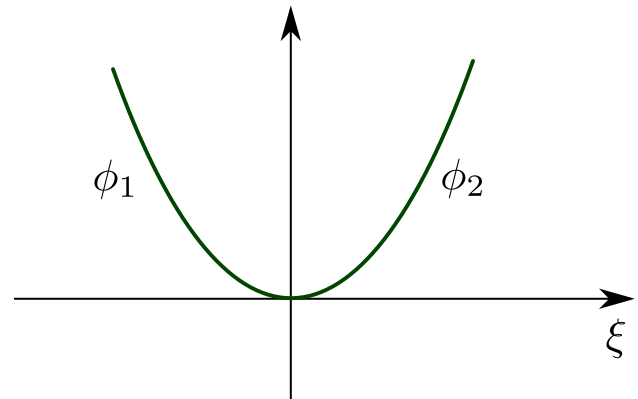
\includegraphics[scale=0.24]{assets/lectures_part_3-7a9fde69.png}
\end{gathered}
$$
\textbf{Тоді: } \fbox{$ f_{\eta} (y) =  \sum\limits_{i = 1}^{ n}{ f_{\xi} (\psi_i (y)) \cdot \left| \psi_i'(y) \right| \cdot \mathbb{I}_{E_{\varphi_i}}(y)}$}.
\end{boxteo}
\begin{proof}
  Розглядаемо множину B.
  $$  \int\limits_{B }^{ }{ f_{\eta} (y)dy} = \mathbb{P} \left\lbrace \eta \in B \right\rbrace =
 \mathbb{P} \left\lbrace \xi \in \phi_1^{-1} (B) \cup \cdots \cup \xi \in \phi_n^{-1} (B) \right\rbrace =
  $$
  $$
  =  \sum\limits_{i = 1}^{n}{ \mathbb{P} \left\lbrace \xi \in \phi_i^{-1} (B) \right\rbrace  }  - \text{ надалі доведення зводиться до попередньої теореми.}
  $$
  \end{proof}

 \subsection{Функції від випадкових векторів.}
 Розглядаємо $ \overline{\xi} = \begin{bmatrix}
  \xi_1 \\
  \xi_2
 \end{bmatrix} \quad \eta = \varphi(\xi_1, \xi_2)$.\\
 1. Для дискретного випадку обчислення тривіальні.\\
 2. $ \overline{\xi} $ - абсолютно неперервний випадковий вектор.
 $$ f_{\overline{\xi}} (\overline{x}) \Rightarrow \eta = \varphi( \overline{\xi}) \quad f_{\eta} (y)=? \quad \varphi: \mathbb{R}^n \to \mathbb{R}$$
\begin{boxteo}
    $ \varphi: \mathbb{R}^n \to \mathbb{R}^n. \varphi$ - взаємно-однозначна $ \Rightarrow \psi = \varphi^{-1}$.\\
    $\varphi, \psi $ - дифеоморфізми $ \Rightarrow  \exists J_{\psi} ( \overline{y}) $ - якобіан. Тоді:
    $$
    f_{\overline{\eta}}  (\overline{y}) = f_{\overline{\xi}} (\psi(\overline{y})) \cdot \left| J_{\psi }(\overline{y}) \right| \cdot   \mathbb{I}_{E_{\varphi}} (\overline{y})
    $$
\end{boxteo}
\begin{boxteo}
    $\varphi$ розпадаэться на суму ін'єктивних функцій  $\varphi_1, ..., \varphi_k$.\\
    $ \varphi^{-1}_i = \psi_i. \quad E_i$ - область значень $ \varphi_i. \quad J_{\psi_i}$ - якобіан $ \psi_i$. Тоді:
    $$
    f_{\eta} (\overline{y}) =  \sum\limits_{i = 1}^{ k}{ f_{\overline{\xi}} ( \psi_i( \overline{y})) \cdot \left| J_{\varphi_i } (\overline{y}) \right|  \cdot \mathbb{I}_{E_{\varphi_i}} (\overline{y})}
    $$
\end{boxteo}
Часто будемо використовувати: \fbox{$f_{\xi_1 + \xi_2} (y) =  \int\limits_{-\infty}^{ +\infty}{ f_{\overline{\xi} } (x, y-x) dx}$}.\\
Якщо $ \xi_1 \independent \xi_2: $ \fbox{$ f_{\xi_1 + \xi_2} (y) =  \int\limits_{-\infty}^{ +\infty}{ f_{\xi_1} (x) \cdot f_{\xi_2} (y-x) dx}$}.\\ Також: $f_{\xi_1 + \xi_2} (y) = (f_{\xi_1} \circledast f_{\xi2} (y))$ - згортка.
\subsection{Загальний алгоритм знаходження щільності функції від випадкових векторів.}
Розглядаємо $ \eta = \varphi( \overline{\xi}) \quad f_{\eta} (z) = ?$.
$$
F_{\eta} = \mathbb{P} \left\lbrace  \eta < z \right\rbrace = \mathbb{P} \left\lbrace \varphi(\xi_1, \xi_2) < z \right\rbrace = \left| \left\lbrace (x,y) \in \mathbb{R} \bigg| \varphi(x,y) < z \right\rbrace = D_z \right|  =
$$
$$
 =  \iint\limits_{D_z}^{}{f_{\overline{\xi} }(x,y ) dxdy} \Longrightarrow f_\eta (z)  = F_\eta' (z)
$$
Знайдемо щільності розподілу суми, добутку та частки випадкових величин.
$$\xi_1, \xi_2, f_{\overline{\xi} }(x,y) \Longrightarrow f_{\xi_1 + \xi_2} (z), f_{\xi_1 \cdot \xi_2} (x,y), f_{\xi_1/ \xi_2} (x,y) - ?$$
\textbf{Сума:} $ F_{\xi_1 + \xi_2} (z) = \mathbb{P} \left\lbrace \xi_1 + \xi_2 < z \right\rbrace = \mathbb{P} \left\lbrace \overline{\xi} \in D_z \right\rbrace =
  \iint\limits_{D_z}^{ }{ f_{\overline{\xi}} ( x,y) dxdy} =
$
$$
\begin{gathered}
=  \int\limits_{-\infty}^{ +\infty}{ dx  \int\limits_{-\infty}^{ z-x}{f_{\overline{\xi}}(x,y)dy}}\\
 f_{\xi_1 + \xi_2} (z) = \int\limits_{-\infty}^{ +\infty}{ f_{\overline{\xi}} (x, z-x) dx}
\end{gathered}\qquad \quad
\begin{gathered}
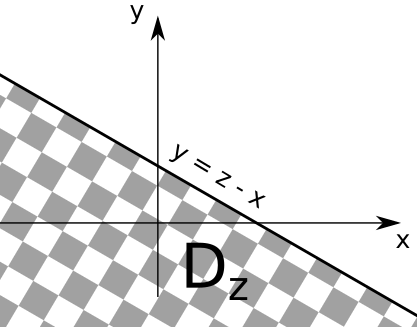
\includegraphics[scale=0.45]{assets/lectures_part_3-43a27a3a.png}
\end{gathered}
$$
$$
f_{\xi_1 + \xi_2} (z) =  \int\limits_{-\infty}^{ +\infty}{ f_{\overline{\xi}}(x, z-x)dx = \left| \xi_1 \independent \xi_2 \right| =  \int\limits_{-\infty}^{ +\infty}{ f_{\xi_1} (x) \cdot f_{\xi_2} (z-x) dx }}
$$
\textbf{Добуток: } Шукаємо $ f_{\xi_1 \cdot \xi_2 } \quad F_{\xi_1 \cdot \xi_2}= \mathbb{P} \left\lbrace \xi_1 \cdot \xi_2 < z \right\rbrace$.\\
$$
\begin{gathered}
x * y < z \Leftrightarrow \left[ \begin{gathered}
\begin{cases}
    y < \frac{z}{x}\\
    x> 0
\end{cases}\\
\begin{cases}
    y > \frac{z}{x}\\
    x < 0
\end{cases}
\end{gathered}
 \right.
\end{gathered}
 \qquad
 \begin{gathered}
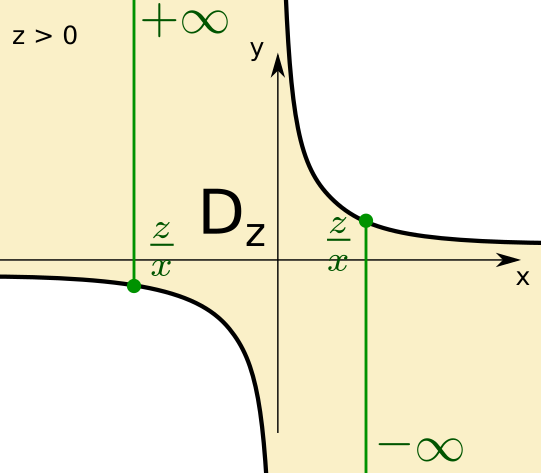
\includegraphics[scale=0.4]{assets/lectures_part_3-5c275c57.png}
 \end{gathered}
$$
$$
F_{\xi_1 \cdot \xi_2} (z) =  \iint\limits_{D_z}^{ }{ f_{\overline{\xi}} (x,y) dxdy} =  \int\limits_{-\infty}^{0}{dx  \int\limits_{ \frac{z}{x}  }^{ +\infty}{ f_{\overline{\xi}} (x,y )dy}} +  \int\limits_{0}^{ +\infty}{ dx  \int\limits_{-\infty}^{ \frac{z}{x} }{f_{\overline{\xi}} (x,y )dy}}
$$
$$
f_{\xi_1 \cdot \xi_2} (z) = -  \int\limits_{-\infty}^{ 0}{ f_{\overline{\xi}}(x, \frac{z}{x})\cdot \frac{1}{x} dx  } + \int\limits_{0}^{ + \infty}{ f_{\overline{\xi}}(x, \frac{z}{x})\cdot \frac{1}{x} dx  }
$$

\textbf{Відношення.} Розглядаємо: $\overline{\xi} = \begin{bmatrix}
 \xi_1 \\
 \xi_2
\end{bmatrix} \quad f_{\overline{\xi}} (x,y) \quad \eta = \frac{\xi_2}{\xi1} $. За алгоритмом:
$$
F_{\eta} (z) = \mathbb{P} \left\lbrace \frac{\xi_2}{\xi_1} <z  \right\rbrace = \mathbb{P} \left\lbrace \overline{\xi} \in D_z \right\rbrace =  \iint\limits_{D_z}^{}{ f_{\overline{\xi}}(x,y)dxdy}
$$
де, $ D_z = \left\lbrace (x,y) \in \mathbb{R}^2| \frac{y}{x} < z  \right\rbrace $
Якщо $z > 0 :$
$$
\begin{gathered}
 \frac{y}{x} < z \Leftrightarrow
\left[
\begin{gathered}
\begin{cases}
    y < xz \\
    x > 0
\end{cases}
\\
\begin{cases}
    y > xz \\
    x < 0
\end{cases}
\end{gathered}
 \right.
 \qquad
\end{gathered}
  \begin{gathered} 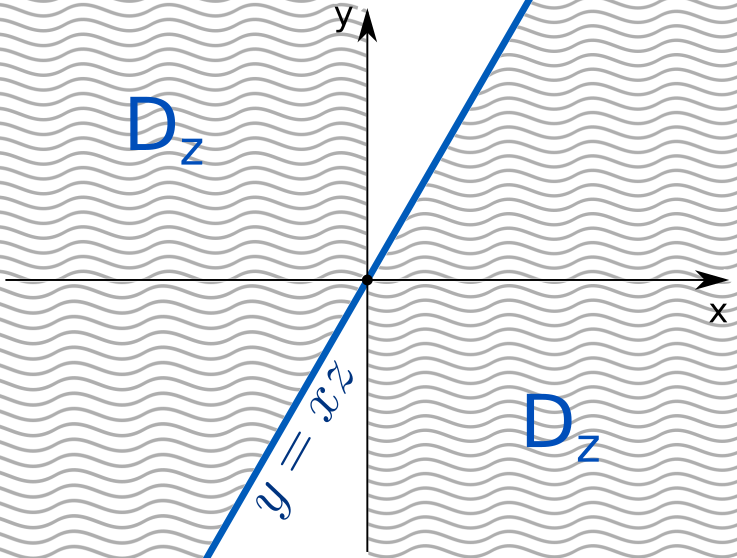
\includegraphics[scale=0.3]{assets/lectures_part_3-f7d7887c.png} \end{gathered}
$$
Повертаємося до інтегралу, що записано вище:
$$
F_{\eta} (z) =  \int\limits_{-\infty}^{0}{ dx   \int\limits_{zx}^{ +\infty}{ f_{\overline{\xi}}}(x,y) dy} +  \int\limits_{0}^{ +\infty}{ dx
 \int\limits_{-\infty}^{zx}{ f_{\overline{\xi}}(x,y) dy}
}
$$
$$
f_{\eta}(z) = F_{\eta}'(z) =  \int\limits_{-\infty}^{ 0}{ f_{\overline{\xi}}(x,zx)x dx} +  \int\limits_{0}^{ +\infty}{f_{\overline{\xi}}(x, zx) x dx}
$$
\begin{example}
    $\xi_1, \xi_2 \sim N(0,1) \quad \xi_1 \independent \xi_2 \quad \eta = \frac{\xi_2}{\xi_1} $
\\ Величини $\xi_1, \xi_2$ розподілені нормально: $
f_{\xi_1} (x) = \frac{1}{\sqrt{2 \pi}} e^{ - \frac{x^2}{2} }  = f_{\xi_2 } (x).
$\\
Скористаємося знайденою формулою:
$$
f_{\eta} (z) = -  \int\limits_{-\infty}^{ 0}{\frac{1}{\sqrt{2 \pi}} e^{ - \frac{x^2}{2} } \cdot \frac{1}{\sqrt{2 \pi}} e^{ - \frac{z^2x^2}{2} } } x dx + \int\limits_{0}^{ +\infty}{\frac{1}{\sqrt{2 \pi}} e^{ - \frac{x^2}{2} } \cdot \frac{1}{\sqrt{2 \pi}} e^{ - \frac{z^2x^2}{2} } } x dx  =
$$
$$
= - \frac{1}{2\pi}  \int\limits_{-\infty}^{0}{ e^{ -\frac{x^2}{2}(1+z^2) }} \underbrace{xdx}_{= d \left( \frac{x^2}{2}  \right)}  + \frac{1}{2\pi}  \int\limits_{0}^{+ \infty}{ e^{ -\frac{x^2}{2}(1+z^2) }} \underbrace{xdx}_{= d \left( \frac{x^2}{2}  \right)} =
$$
$$
= - \frac{1 }{2 \pi ( 1 + z^2)}  \int\limits_{-\infty}^{0}{ e^{- \frac{x^2}{2}(1+z^2) } d \left( \frac{x^2}{2}(1+z^2) \right) }  + \frac{1 }{2 \pi ( 1 + z^2)}  \int\limits_{0}^{+ \infty}{ e^{- \frac{x^2}{2}(1+z^2) } d \left( \frac{x^2}{2}(1+z^2) \right) } =
$$
$$
= \frac{1 }{2 \pi ( 1 + z^2)}   e^{- \frac{x^2}{2}(s+z^2) } \Bigg|_{x = -\infty}^{0}  - \frac{1 }{2 \pi ( 1 + z^2)}   e^{- \frac{x^2}{2}(1+z^2) } \Bigg|_{x = 0}^{+\infty} =
$$
$$
 =\frac{1}{2\pi (1+ z^2)} +  \frac{1}{2\pi (1+ z^2)} = \frac{1}{\pi (1+ z^2)} , z \in \mathbb{R}
$$
Отримали, що: $ \dfrac{N(0,1)}{N(0,1)} \sim \textbf{Cauchy Distribution} $
\end{example}

\subsection{Щільності розподілу максимума, мінімума та інших порядкових статистик.}
\subsubsection{Максимум.}
Розглянемо максимум з деяких незалежних випадкових величин: $ \xi_1 , \xi_2, ... , \xi_n$.
$$M = \max \left\lbrace \xi_1, ..., \xi_n \right\rbrace $$
$$
F_M (x) =  \mathbb{P} \left\lbrace M < x \right\rbrace = \mathbb{P} \left\lbrace \max \left\lbrace \xi_1, ... , \xi_n \right\rbrace < x  \right\rbrace  = \mathbb{P} \left\lbrace \xi_1 < x, ... , \xi_n < x \right\rbrace =
$$
$$
= \mathbb{P} \left\lbrace \xi_1 M x \right\rbrace \cdot ... \cdot \mathbb{P} \left\lbrace  \xi_n < x \right\rbrace = F_{\xi_1} (x ) \cdot ... \cdot F_{\xi_n} (x)
$$
\begin{center}
    \fbox{$
    F_M (x) = \prod\limits_{i=1}^{n} F_{\xi_i}(x)
    $}
\end{center}
Якщо $\xi_1 , ..., \xi_n$ однаково розподілені, то $ F_M (x) = F^n_{\xi} (x)$. В такому випадку, можемо знайти і функцію розподілу: $ f_M (x) = n \cdot F_{\xi}^{n-1} (x) \cdot f_{\xi }(x)$.
\subsubsection{Мінімум.}
Розглянемо мінімум з деяких незалежних випадкових величин: $ \xi_1 , \xi_2, ... , \xi_n$.
$$m = \min \left\lbrace \xi_1, ..., \xi_n \right\rbrace $$
$$ F_m (x) = \mathbb{P} \left\lbrace  \min{\xi_1, ..., \xi_n} < x\right\rbrace = 1 - \mathbb{P} \left\lbrace \min{\xi_1, ..., \xi_n} \geq  x \right\rbrace =
$$
$$
=  1 - \mathbb{P} \left\lbrace \xi_1 \geq x, ... , \xi_n \geq x  \right\rbrace  = 1 - \left( 1 - F_{\xi_1} (x) \right) \cdot ... \cdot \left( 1 - F_{\xi_n} (x) \right)
$$
\begin{center}
    \fbox{$
    F_m (x) =1 - \prod\limits_{i=1}^{n}\left(  1- F_{\xi_i}(x) \right)
    $}
\end{center}
Якщо $\xi_1 , ..., \xi_n$ однаково розподілені, то $ F_m (x) = 1 - \left(  1- F_{\xi}(x) \right)^{n} $. В такому випадку, можемо знайти і функцію розподілу: $ f_m (x) = n \cdot \left( 1 - F_{\xi}(x) \right)^{n-1}  \cdot f_{\xi }(x)$.
\subsubsection{Порядкові статистики.}
$ \xi_1 , \xi_2 ... , \xi_n $ - незалежні однаково розподілені абсолютно неперерні випадкові величини зі щільністью $f$.
Знайдемо: $ \mathbb{P} \left\lbrace \xi_i - \xi_j = 0 \right\rbrace  = 0 \Leftrightarrow \mathbb{P} \left\lbrace \xi_i \neq \xi_j \right\rbrace = 1$. \\
Це означає, що з імовірністю 1 всі величини різні. Тому, можемо впорядкувати величини за зростанням:
$$
\underbrace{\xi_{(1)}}_{\min{\left\lbrace \xi_1, ..., \xi_n \right\rbrace }} \quad < \quad \xi_{(2)} \quad < \quad \cdots \quad < \quad \underbrace{\xi_{(n)}}_{\max{\left\lbrace \xi_1, ..., \xi_n \right\rbrace }}
$$
$ \xi_{(k)}, k \in [1, n]$ - k-та порядкова статистика (order statistics).\\
Щільність розподілу $\xi_{(k)}, k \in [1,n]:$
$$
F_{\xi_{(k)}}  (x) = \mathbb{P} \left\lbrace \xi_{(k)} < x \right\rbrace = \mathbb{P} \left\lbrace \forall i \leq k : \xi_i \in (-\infty, x) \right\rbrace =
$$
$$
=  \sum\limits_{l = k}^{n}{
\underbrace{\mathbb{P} \left\lbrace n( \xi_i \in (-\infty, x)) = l \right\rbrace}_{\text{схема Бернуллі}}
}=\sum\limits_{l = k}^{ n}{ C^l_n \cdot F^l(x) \cdot \overline{F}^{n-l}(x)}
$$
$$
f_{\xi_{(k)}} (x) = F_{\xi_{(k)}}'  (x) =  \sum\limits_{l = k}^{n}{ C^l_n \left(
l  F^{l-1} (x) f(x) \overline{F}^{n-l} (x) - F^l (x)(n-l) \overline{F}^{n-l-1}(x)  f(x)
 \right) }=
$$
$$
= \left| \begin{gathered}
 \text{Телескопічна сума.}\\
 \text{Доданки скорочуються.}\\
\end{gathered} \right| = \frac{n!}{(k-1)! (n-k)!} F^{k-1}(x) \cdot \overline{F}^{n-k}(x) \cdot f(x), k \in [1,n]
$$

\newpage

\subsection{Знаходження числових характеристик функцій від випадкових величин.}

\begin{boxteo}
Нехай є випадковий вектор $\overline{\xi} = \begin{bmatrix}
 \xi_1 \\
 \vdots \\
 \xi_n
\end{bmatrix}$. Та фукнція $\varphi: \mathbb{R}^n \to \mathbb{R}$. В такому вигляді, ми не можемо застосувати теорему до характеристичної функції, адже характеристична функція є комплекснозначною. Але, слід зауважити, що умови теореми будуть виконуватися і в комплексному випадку.
$$
\mathbb{E} \varphi(\overline{\xi}) = \underset{R^n}{ \int \cdots \int} \varphi (x_1, ..., x_n) \cdot f_{\overline{\xi}}(x_1, ..., x_n)dx_1 \cdots dx_n
$$
\end{boxteo}

\begin{proof}
   Для 2-вимірного випадку. Дано:
   $$
   n=2 \qquad \overline{\xi}= \begin{bmatrix}
    \xi_1 \\
    \xi_2
   \end{bmatrix} \qquad \eta = \varphi(\xi_1 , \xi_2)
   $$
   Доведемо, що: $\mathbb{E} \varphi (\xi_1, \xi_2) =  \int\limits_{- \infty}^{ +\infty}{  \int\limits_{-\infty}^{ +\infty}{
   \varphi(x,y) f_{\overline{\xi}} (x,y)dxdy
   }}$\\
   Спочатку доведемо одну допоміжну лему.\\
   \textbf{Лема. } $\mathbb{P} \left\lbrace \eta \geq 0 \right\rbrace = 1 \Longleftrightarrow \eta \geq 0$ м.н (a.s.). \textbf{Тоді }
   $\mathbb{E} \eta  =  \displaystyle\int\limits_{0}^{ +\infty}{\underbrace{\overline{F_\eta} (x) dx}_{1 - F_\eta (x) = \mathbb{P} \left\lbrace \eta \geq x \right\rbrace}}$.
   \begin{proof} (леми)
   $$
   \begin{gathered}
    \text{Раніше, за означенням:}\\
     \mathbb{E} \eta =  \int\limits_{0}^{ +\infty}{x \cdot f_{\eta} (x) dx }
   \end{gathered} \quad \Longleftrightarrow \quad
   \begin{gathered}
    \text{Більш загально:}\\
     \mathbb{E} \eta  =  \int\limits_{0}^{ +\infty}{\overline{F_\eta} (x) dx}
   \end{gathered}
   $$
   $$
   \eta =  \int\limits_{0}^{\eta}{1 dx} =  \int\limits_{0}^{ +\infty}{ \ind{}\left\lbrace \eta \geq x \right\rbrace dx}
\quad \Longrightarrow \quad
\mathbb{E} \eta = \mathbb{E} \int\limits_{0}^{ +\infty}{ \ind{}\left\lbrace \eta \geq x \right\rbrace dx} =
   $$
   Можемо внести математичне сподівання під знак інтегралу.
   $$
   =  \int\limits_{0}^{ +\infty}{\underbrace{ \mathbb{E}\ind{}\left\lbrace \eta \geq x \right\rbrace}_{ \mathbb{P} \left\lbrace \eta \geq x \right\rbrace} dx} =  \int\limits_{0}^{ +\infty}{ \mathbb{P} \left\lbrace \eta \geq x \right\rbrace} dx =  \int\limits_{0}^{ +\infty}{\overline{F_\eta} (x) dx}
   $$
   \end{proof}
   Повернемося до доведення основної теореми. Нехай $ \varphi(x,y) \geq 0 \quad \forall (x,y) \in \mathbb{R}^2.$
   $$
   \mathbb{E} \eta = \underbrace{\mathbb{E} \varphi (\xi_1, \xi_2)}_{ \geq 0 } =  \int\limits_{0}^{ +\infty}{\mathbb{P} \left\lbrace \varphi(\xi_1, \xi_2) \geq z  \right\rbrace dz} =
     D_z : \left\lbrace (x,y) \in \mathbb{R}^2 \big| \varphi(x,y) \geq z \right\rbrace =
    $$
    $$
    =  \int\limits_{0}^{ +\infty}{\mathbb{P} \left\lbrace \overline{\xi} \in D_z \right\rbrace} =  \int\limits_{0}^{ +\infty}{ \left( \iint\limits_{D_z} f_{\overline{\xi}}(x,y)  dxdy \right) } dz =  \iint\limits_{R^2}{ f_{\overline{\xi}}(x,y) \left( \int\limits_{0}^{ \varphi(x,y)} dz  \right) }dxdy =
    $$
    $$
    = \iint\limits_{\mathbb{R}^2} \varphi(x,y)\cdot f_{\overline{\xi}} (x,y) dxdy
    \quad \text{Що і треба було показати.}
    $$
Нехай $\varphi(x,y)$ - довільна. Скористаємося фактом, що будь-яку функцію можна зобразити як різницю двох невід'ємних функцій:
$$
\varphi(x,y) = \varphi_+ (x,y) - \varphi_{-} (x,y) \qquad \begin{gathered}
 \varphi_+ (x,y)  = \max \left\lbrace \varphi(x,y), 0 \right\rbrace \geq  0\\
  \varphi_{-} (x,y) = - \min \left\lbrace \varphi(x,y), 0 \right\rbrace \geq 0
\end{gathered}
$$
$$
\begin{gathered} 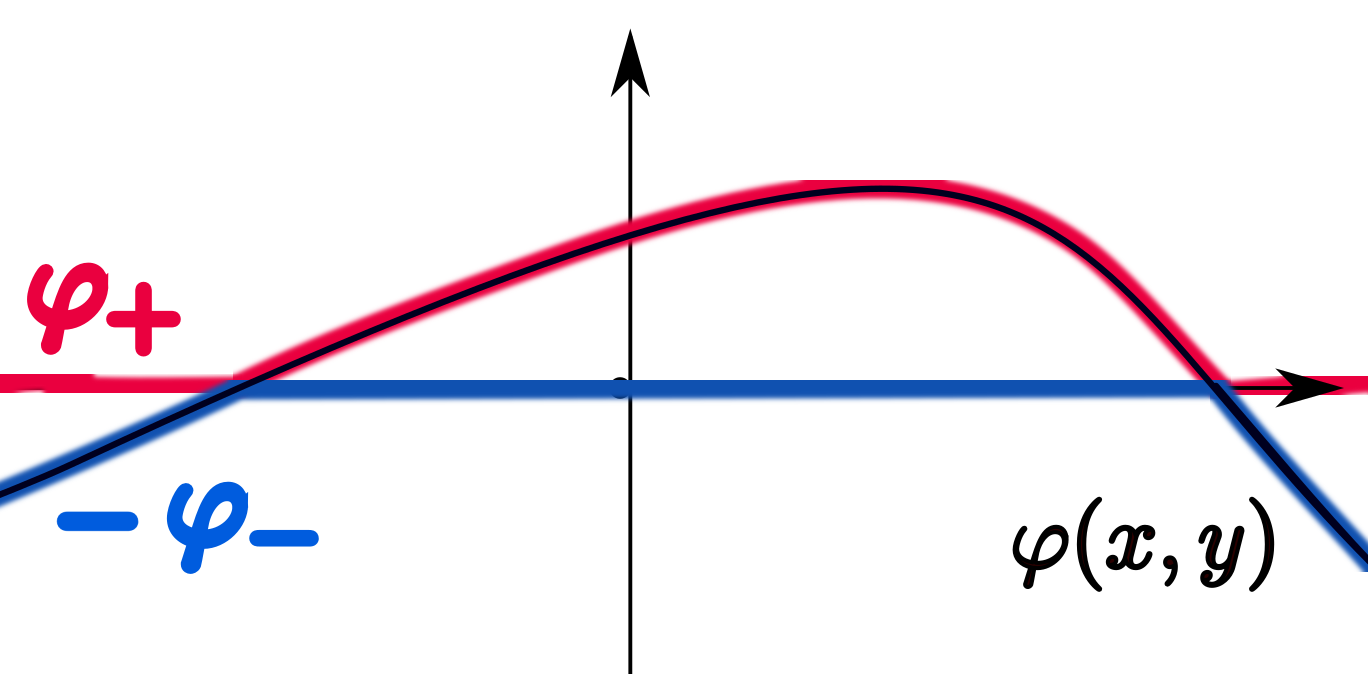
\includegraphics[scale=0.18]{assets/lectures_part_3-571a6e75.png} \end{gathered}
\qquad
\begin{gathered}
 \underbrace{ \varphi_+ + (- \varphi_- )}_{\varphi_+ - \varphi_-}= \Bigg[ \begin{gathered}
  \varphi + 0\\
  0 + \varphi
 \end{gathered} = \varphi
\end{gathered}
$$
$$
\mathbb{E} \eta = \mathbb{E} \varphi(\xi_1, \xi_2) = \mathbb{E} \left(  \varphi_+ (\xi_1, \xi_2) - \varphi_- (\xi_1, \xi_2) \right) =\mathbb{E} \varphi_+ (\xi_1, \xi_2) -  \mathbb{E} \varphi_- (\xi_1, \xi_2) \circled{=}
$$
{\small  Застосовуємо висновок про математичне сподівання невід'ємної функції:}
$$
 \circled{=} \iint\limits_{\mathbb{R}^2} \varphi_+(x,y) f_{\overline{\xi}} (x,y)dxdy - \iint\limits_{\mathbb{R}^2} \varphi_-(x,y) f_{\overline{\xi}} (x,y)dxdy =
$$
$$
= \iint\limits_{\mathbb{R}^2} \left( \varphi_+ (x,y) - \varphi_- (x,y)  \right) f_{\overline{\xi}} (x,y) dxdy =
\iint\limits_{\mathbb{R}^2} \varphi(x,y) f_{\overline{\xi}} (x,y) dxdy \quad \text{ Ч.и.т.д.}
$$

\end{proof}

\newpage

\section{Деякі ймовірнісні розподіли, що зустрічаються у математичній статистиці.}

\subsection{Гамма-розподіл.}
\subsubsection{PDF.}
Будемо називати гамма розподіленою величиною $\xi \sim \gammadistr(\alpha, \beta)\quad \alpha , \beta >0$:
$$
\begin{gathered}
f_{\xi}(x) = \begin{dcases}
     \frac{\beta^{\alpha}}{\Gamma(\alpha)} x^{\alpha-1}e^{-\beta x}, & x > 0;\\
    0, & x\leq  0;
\end{dcases}
\end{gathered} \qquad  \begin{gathered}
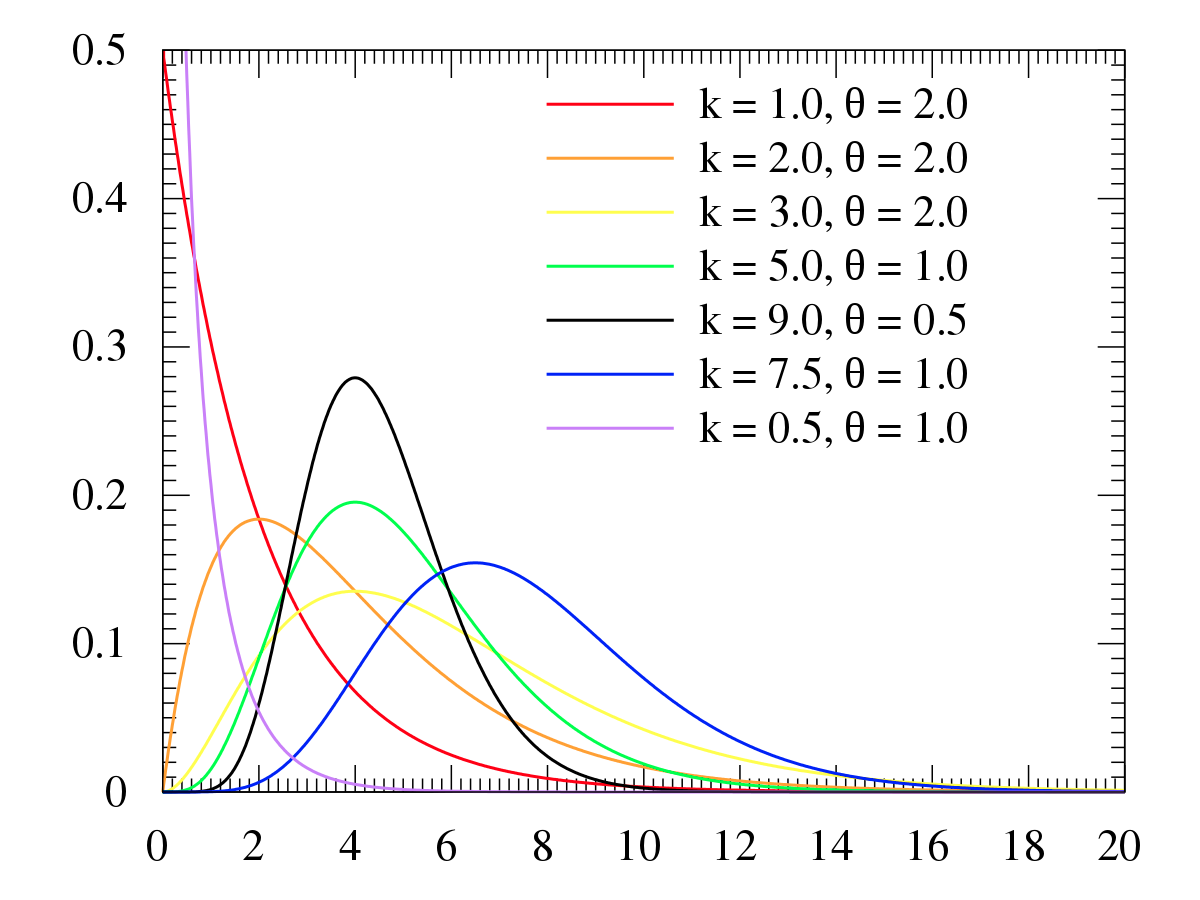
\includegraphics[scale=0.2]{assets/lectures_part_3-f657bbe5.png}
\end{gathered}
$$

За умовою нормування:
$$
1 = c  \int\limits_{9}^{ +\infty}{ x^{\alpha-1}e^{-\beta x} dx} = \frac{c}{\beta^\alpha}  \underbrace{ \int\limits_{0}^{ +\infty}{ (\beta x)^ {\alpha -1 } e^{\beta x} d (\beta x)}}_{\gammadistr{(\alpha)}}   = \frac{c \cdot \Gamma(\alpha)}{\beta^{\alpha}}  \Longrightarrow c = \frac{\beta^{\alpha}}{\Gamma(\alpha)}
$$
Розглянемо випадок $\alpha =  1$: \qquad  $f_{\Gamma(1, \beta)} (x) = \begin{dcases}
 \beta e^{-\beta x }, & x > 0 ;\\
 0, & x\leq  0 ;
\end{dcases} = f_{Exp(\beta)}$\\
Тобто, экспоненціальний розподіл є окремим випадком гамма-розподілу.
\subsubsection{Числові характеристики.}
Знайдемо одразу n-тий момент величини $ \xi \sim \Gamma(\alpha, \beta)$.
$$
\mathbb{E} \xi^n =  \int\limits_{0}^{ +\infty}{ x^n \cdot f_{\xi} (x) dx} =  \int\limits_{0}^{ +\infty}{x^n  \frac{\beta^{\alpha}}{\Gamma(\alpha)} x^{\alpha-1}e^{-\beta x}}dx = \frac{\beta^{\alpha}}{\Gamma(\alpha)} \cdot   \int\limits_{0}^{ +\infty}{ x^{\alpha+n-1}e^{-\beta x}}dx =
$$
$$
=  \frac{\beta^{\alpha}}{\Gamma(\alpha) \cdot \beta^{n + \alpha}} \cdot   \int\limits_{0}^{ +\infty}{ \left( \beta x \right) ^{\alpha+n-1}e^{-\beta x}} d \left( \beta x \right)  = \fbox{$ \dfrac{\Gamma(\alpha + n)}{ \beta^n \cdot \Gamma(\alpha)}$}
$$
$
\mathbb{E} \xi = (n = 1 ) = \frac{1}{ \beta \cdot \Gamma (\alpha)} \cdot \Gamma(\alpha+1) = \frac{\alpha}{\beta}
$\\
$
\mathbb{E} \xi^2 = (n = 2) = \frac{1}{\beta^2 \cdot \Gamma (\alpha) }  \cdot \Gamma(\alpha + 2) = \frac{\alpha ( \alpha + 1)}{\beta^2}
$\\
$
\mathbb{D} \xi = \mathbb{E}(\xi^2) - \left( \mathbb{E}\xi \right) ^2 = \frac{\alpha ( \alpha + 1)}{\beta^2} - \frac{\alpha^2}{\beta^2} = \frac{\alpha}{\beta^2}
$
\subsubsection{Стійкість відносно додавання.}

Як ми пам'ятаємо, експоненціальний розподіл не є стійким відносно додавання. Тобто, при додаванні двох експоненціальних випадкових величин між собою, результат не буде експоненціальною величиною. Але, як вже відомо, експоненціальний розподіл належить до більш широкого класу - гамма-розподілів. Таким чином, є сенс дослідити, чи будемо ми за афінних перетворень залишатися всередині класу гамма-розподілів.
\begin{boxteo}[Про напівстійкість Гамма-розподілу.]
$$
 \independent \begin{cases}
  \xi_1 \sim \Gamma (\alpha_1, \beta)\\
  \xi_2 \sim \Gamma (\alpha_2, \beta)
\end{cases} \quad \Longrightarrow \quad \fbox{$ \xi_1 + \xi_2 \sim \Gamma(\alpha_1 + \alpha_2 , \beta)$}
$$
\end{boxteo}

\begin{proof} За умовою, маємо:
 $$
 f_{\xi_1} = \begin{dcases}
      \frac{\beta^{\alpha_1}}{\Gamma(\alpha_1)} x^{\alpha_1-1}e^{-\beta x}, & x > 0;\\
     0, & x\leq  0;
 \end{dcases} \qquad \qquad  f_{\xi_2} = \begin{dcases}
       \frac{\beta^{\alpha_2}}{\Gamma(\alpha_2)} x^{\alpha_2-1}e^{-\beta x}, & x > 0;\\
      0, & x\leq  0;
  \end{dcases}
 $$
 $$
 \text{Скористаємося правилом згортки: }\quad f_{\xi_1 + \xi_2} (y) =  \int\limits_{-\i }^{ +\infty}{ f_{\xi_1 } (x) f_{\xi_2} (y-x) dx} =
 $$
 $$ = \textstyle{\frac{\beta^{\alpha_1}\beta^{\alpha_2}}{\Gamma{(\alpha_1)}  \Gamma(\alpha_2)} }  \displaystyle\int\limits_{0}^{y}{
 x^{\alpha_1 - 1 } e^{- \beta x} (y-x)^{\alpha_2 - 1} e^{-\beta(y-x)}dx
 }
=
 \left|
\underbrace{\begin{cases}
 x > 0 \\
 y - x > 0
\end{cases}\begin{cases}
 x > 0\\
 x < y
\end{cases}}_{x \in(0, y)}
  \right| \circled{=}
 $$
 Зауваження. Надалі будемо вважати, що при $y\leq 0 \quad f_{\xi_1 + \xi_2 } (y) =0$.
 $$
 \circled{=} \frac{\beta^{\alpha_1 + \alpha_2} e^{-\beta y}}{ \Gamma(\alpha_1) \Gamma(\alpha_2)}  \int\limits_{0}^{y}{x^{\alpha_1 - 1} (y -x)^{\alpha^2 -1 }dx} = \left| \begin{gathered}
   x = y t \quad dx = ydt\\
   x :  0 \to y \\
   t : 0 \to  1
 \end{gathered} \right|  =
 $$
 $$
 = \frac{\beta^{\alpha_1 + \alpha_2} e^{-\beta y}}{ \Gamma(\alpha_1) \Gamma(\alpha_2)}  \int\limits_{0}^{1}{ y^{\alpha_1 - 1} t^{\alpha_1 - 1} y^{\alpha_2 - 1} (1-t)^{\alpha_2 -1 }ydt } =
 $$
 $$
 =  \frac{\beta^{\alpha_1 + \alpha_2} e^{-\beta y}}{ \Gamma(\alpha_1) \Gamma(\alpha_2)} \cdot y^{\alpha_1 + \alpha_2 - 1} \cdot \underbrace{\int\limits_{0}^{1}{t^{\alpha_1 - 1} (1 - t )^{\alpha_2 -1} dt} }_{\beta(\alpha_1 , \alpha_2)= \frac{\Gamma(\alpha_1)\Gamma(\alpha_2)}{\Gamma(\alpha_1+ \alpha_2)} }= \frac{\beta^{\alpha_1 + \alpha_2} e^{-\beta y}}{ \Gamma(\alpha_1 + \alpha_2)} \cdot y^{\alpha_1 + \alpha_2 - 1} =
 $$
 $$
 = \begin{dcases}
   \frac{\beta^{\alpha_1 + \alpha_2}}{ \Gamma(\alpha_1 + \alpha_2)} \cdot y^{\alpha_1 + \alpha_2 - 1} e^{-\beta y}, & y > 0;\\
   0 & y \leq 0;
 \end{dcases} = f_{\Gamma(\alpha_1 + \alpha_2 , \beta)} (y)
 $$
\end{proof}

\subsection{Chi-square distribution with n degrees of freedom.}
\subsubsection{PDF.}
Розглядаємо $\xi_1 ,..., \xi_n $ - незалежні гаусівські $N(0,1)$. Інакше: $ \overline{\xi} = \begin{bmatrix}
 \xi_1 \\
 \vdots\\
 \xi_n
\end{bmatrix} \sim N(\vec{0}, I)$.
Розподіл $ \chi^2_n $ - це закон розподілу $ \left| \left| \overline{\xi} \right|  \right|^2 =  \sum\limits_{i = 1}^{n}{\xi_i^2}$.\\
$
n = 1.$ Шукаємо: $  \xi^2, \xi \sim N(0,1)$.
$$
\varphi(x)  = x^2 \quad x^2 = y \Longrightarrow x = \pm \sqrt{y} \Longrightarrow \begin{gathered}
\psi_1(y) = - \sqrt{y}\\
\psi_2 (y) = \sqrt{y}
\end{gathered} \quad E_{\varphi_1} = \mathbb{E}_{\varphi_2} = [0, + \infty]
$$
$$
f_{\varphi(\xi)} (y) =  \sum\limits_{i = 1}^{2}{ f_{\xi}} \left( \psi_i (y) \right)  \cdot \left| \psi'_i(y) \right| \cdot \ind{}\left\lbrace y \in E_{\varphi_i} \right\rbrace
 =
 $$
 $$
 = \frac{1}{ \sqrt{2 \pi} } e^{- \frac{x^2}{2} } \bigg|_{x = -\sqrt{y}} \cdot \left| \left( - \sqrt{y} \right)'  \right| \cdot \ind{R_+} (y)  +  \frac{1}{ \sqrt{2 \pi} } e^{- \frac{x^2}{2} } \bigg|_{x = \sqrt{y}} \cdot \left| \left( \sqrt{y} \right)'  \right| \cdot \ind{R_+} (y) =
 $$
 $$
 = \frac{2}{ \sqrt{2 \pi} } e^{- \frac{y}{2} } \cdot \frac{1}{ 2 \sqrt{y}} \cdot \ind{R_+} (y) = \begin{cases}
  \frac{1}{\sqrt{2\pi}} y^{- \frac{1}{2} } \cdot e^{ - \frac{1}{2}y}, & y > 0; \\
  0 , & y \leq  0
 \end{cases}   = f_{ \chi_1 ^2} (y)
 $$
$n \in \mathbb{N}.$ Шукаємо: $ \sum\limits_{i = 1}^{n}{\xi_i^2}  \quad \forall \xi_i  : \xi_i \sim N(0,1)$.\\
Розглянемо щільність $ f_{ \chi_1 ^2} (y)$:
$$
\begin{dcases}
\frac{1}{\sqrt{2\pi}} y^{- \frac{1}{2} } \cdot e^{ - \frac{1}{2}y}, & y > 0; \\
0 , & y \leq  0
\end{dcases} =
\begin{dcases}
 \frac{\left( \frac{1}{2} \right) ^{ 1/2 }}{\Gamma \left(  \frac{1}{2}  \right) }  y^{ \frac{1}{2}  - 1} e^{ - \frac{1}{2} y } , & y > 0; \\
 0 , & y \leq  0
\end{dcases} \quad \begin{gathered}
 \text{Впізнаємо гамма-розподіл:}\\
 \chi_1^2 \sim \Gamma \left( \frac{1}{2} ; \frac{1}{2}  \right)
\end{gathered}
$$
Тоді, $\chi^2_n$ це сумма n-незалежних $\chi_1^2$: $\chi^2_n = \underbrace{\chi_1^2 + ... + \chi_1^2}_{n} = \Gamma \left(  \frac{n}{2}, \frac{1}{2} \right)  $
$$
f_{
\chi_n^2
} (x) = \begin{dcases}
 \frac{ \frac{1}{2}^{ \frac{n}{2}  }  }{ \Gamma \left(  \frac{n}{2}  \right) } x^{ \frac{n}{2} -1  } e^{- \frac{1}{2}x }, & x > 0;\\
 0 , & x \leq 0;
\end{dcases}  =
\begin{dcases}
\frac{ 1 }{2^{ \frac{n}{2}  }  \Gamma \left(  \frac{n}{2}  \right) } x^{ \frac{n}{2} -1  } e^{- \frac{x}{2} }, & x > 0;\\
0 , & x \leq 0;
\end{dcases}
$$
$n = 2.$ Зокрема, в такому випадку, отримаємо: $ \chi_2^2 = \Gamma \left( 1, \frac{1}{2}  \right) = Exp \left( \frac{1}{2} \right)  $.
\begin{center}
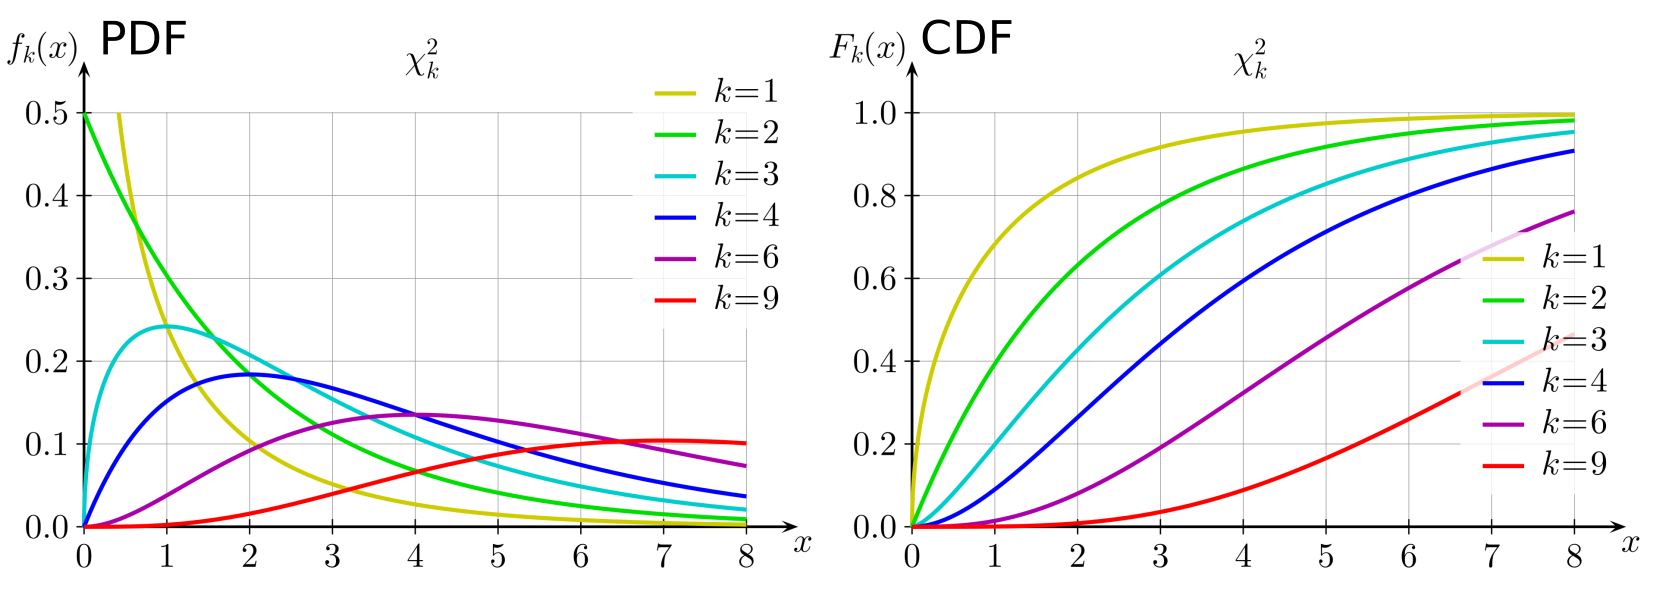
\includegraphics[scale=0.3]{assets/lectures_part_3-d1334d87.png} 
\end{center}
\subsubsection{Числові характеристики.}
$\mathbb{E} \chi^2_n = \mathbb{E} \Gamma \left( \frac{1}{2} , \frac{1}{2}   \right) = n  \quad \left[ \mathbb{E} \left( \xi_1^2 + ... \xi_n^2 \right) = \mathbb{E} \xi_1^2 + ... + \mathbb{E}\xi_n^2 = n \right]$\\
$\mathbb{D} \chi^2_n = \mathbb{D} \Gamma \left( \frac{1}{2} , \frac{1}{2}   \right) = 2n $
